\documentclass{article}

% Librerie 
\usepackage[utf8]{inputenc}
\usepackage[T1]{fontenc}
\usepackage[italian]{babel}
\usepackage{graphicx}
\usepackage{lipsum}
\usepackage{fancyhdr}
\usepackage{titlesec}
\usepackage{tocloft}
\usepackage{titling}
\usepackage{geometry}
\usepackage{float} % Per utilizzare l'opzione H
\usepackage{caption}


% Formattare codice
\usepackage{listings}
\lstset{language=Python}

% Citazioni 
\usepackage[backend=biber, style=verbose]{biblatex}
\addbibresource{cit.bib}


% Configurazione immagini
\captionsetup[figure]{name=Figura}


% Margini
\geometry{a4paper, margin=2cm}

% Titolo
\title{Alberi binari di Ricerca con chiavi duplicate}
\author{Niccolò Caselli}
\date{20/01/2024}
\renewcommand{\maketitlehooka}{\centering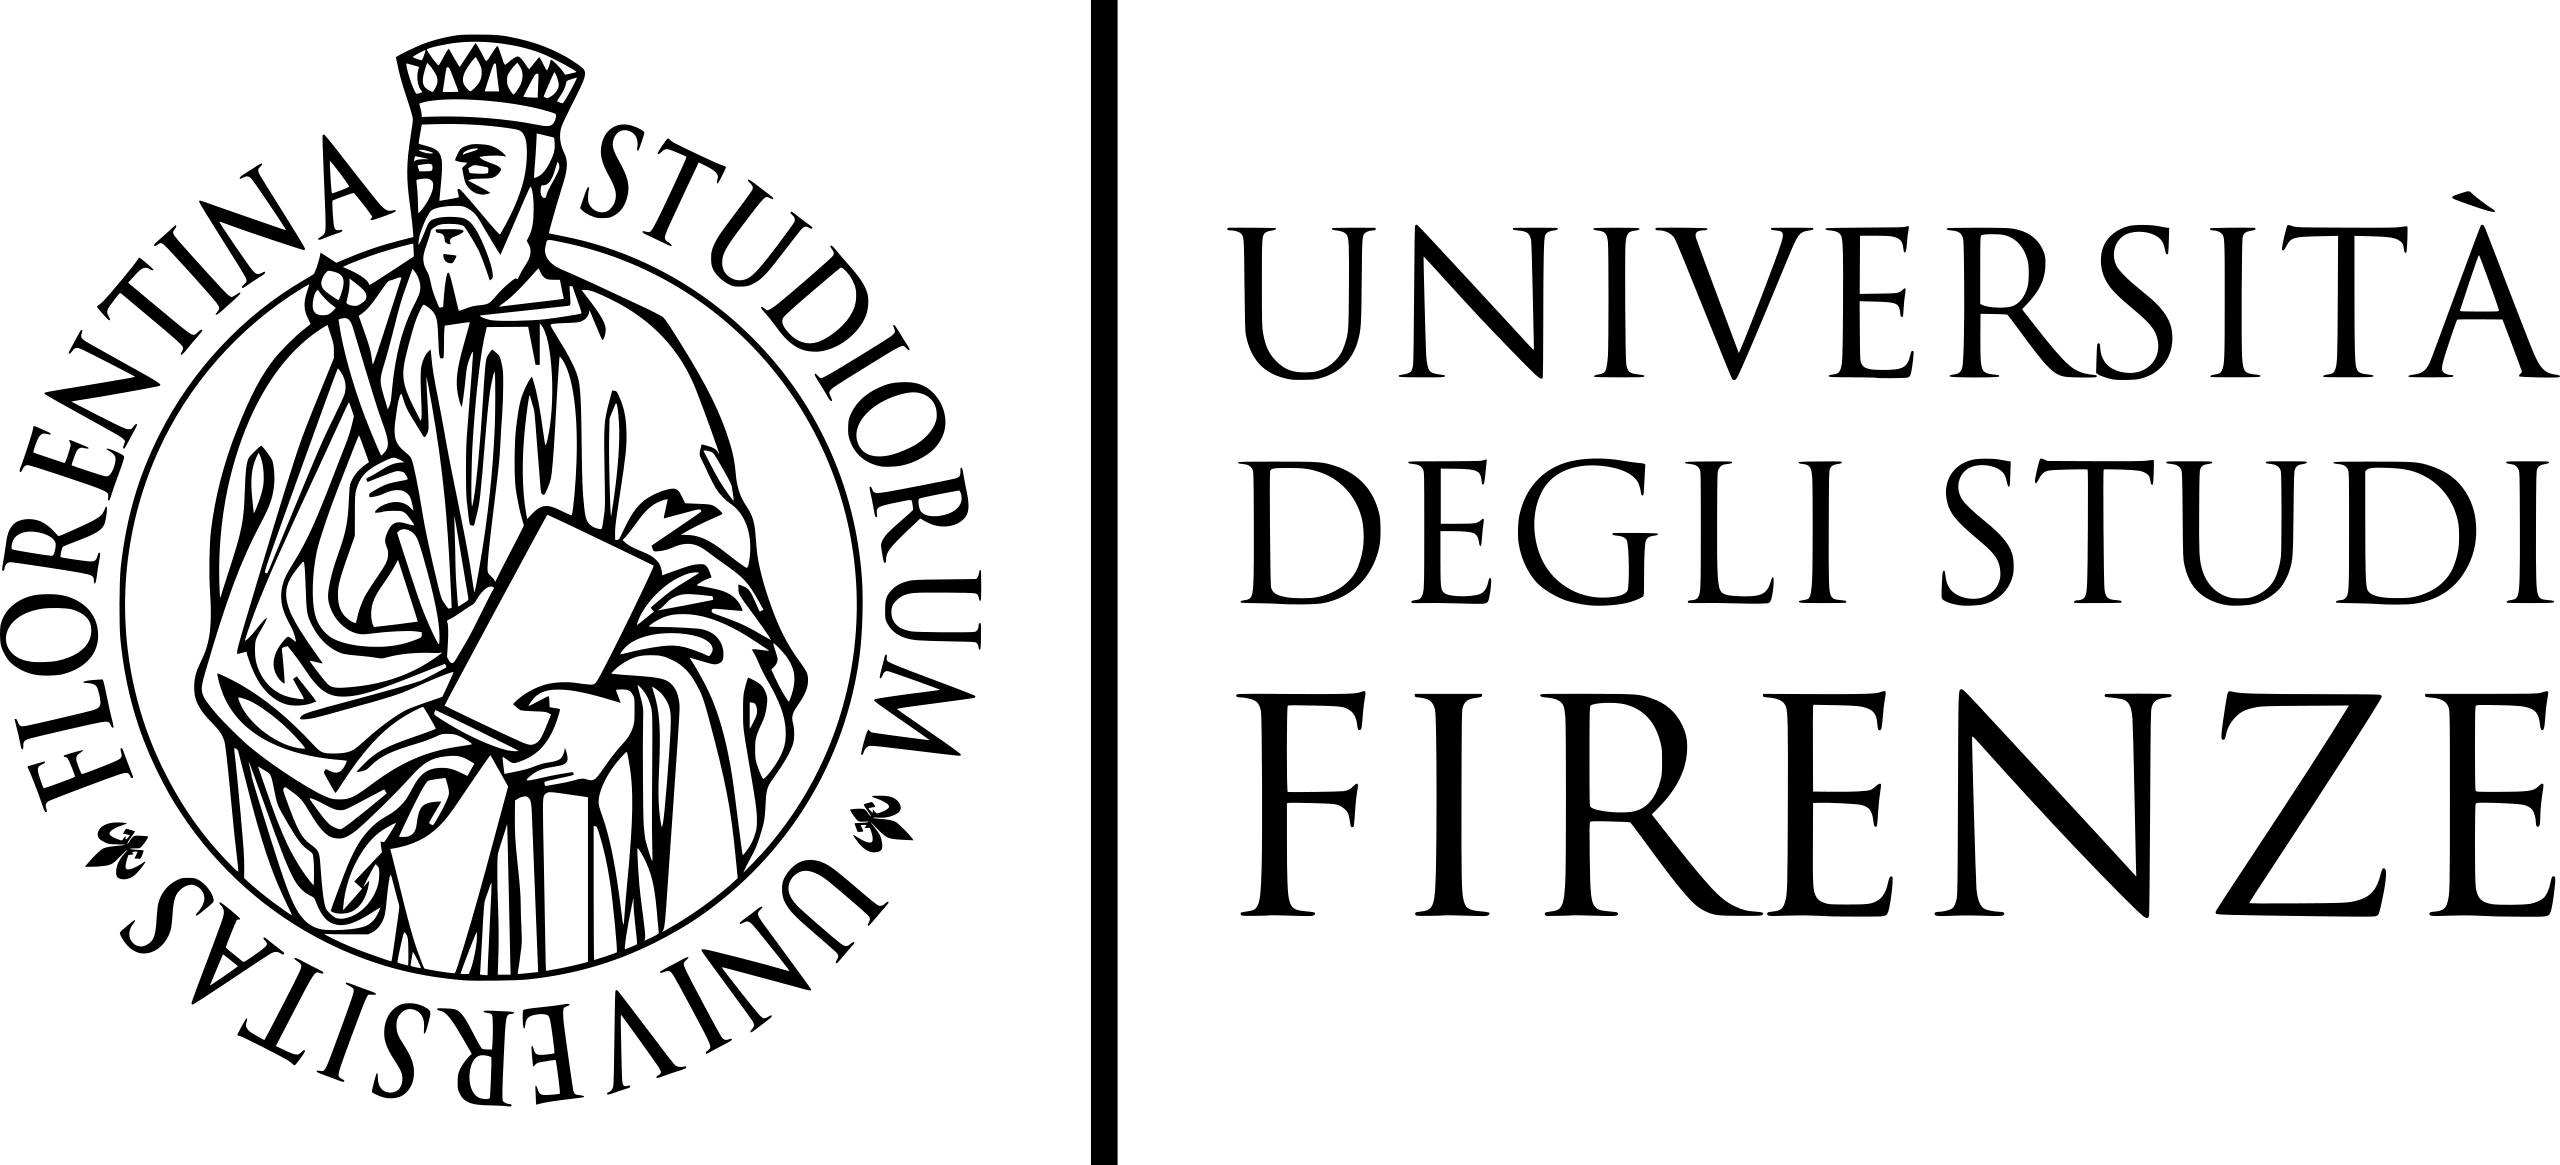
\includegraphics[width=0.5\textwidth]{logo}\vspace{1cm}}
\renewcommand{\maketitlehookb}{\centering\LARGE}
\renewcommand{\maketitlehookc}{\vspace{1cm}\centering\Large}

% Indice
\renewcommand{\cftsecleader}{\cftdotfill{\cftdotsep}}
\setlength{\cftbeforesecskip}{8pt}

% Configurazione degli stili di pagina
\pagestyle{fancy}
\fancyhf{}
\rhead{\thepage}
\lhead{\nouppercase{\leftmark}}
\renewcommand{\headrulewidth}{0.4pt}
\renewcommand{\footrulewidth}{0.4pt}

% Configurazione dei titoli delle sezioni
\titleformat{\section}[block]{\normalfont\Large\bfseries}{\thesection}{1em}{}
\titlespacing*{\section}{0pt}{\baselineskip}{\baselineskip}




\begin{document}

% PAGINA INIZIALE
\begin{titlepage}
  \maketitle
  \vspace*{\fill}
  \begin{center}
    \textbf{Progetto di Laboratorio di Algoritmi e Strutture Dati}
  \end{center}
  \vspace*{\fill}
\end{titlepage}


% INDICE
\renewcommand{\contentsname}{Indice} % Titolo dell'indice
\tableofcontents
\newpage

\section{Introduzione}
\lipsum[1]


\section{Alberi Binari di Ricerca}

\begin{figure}[H]
  \centering
  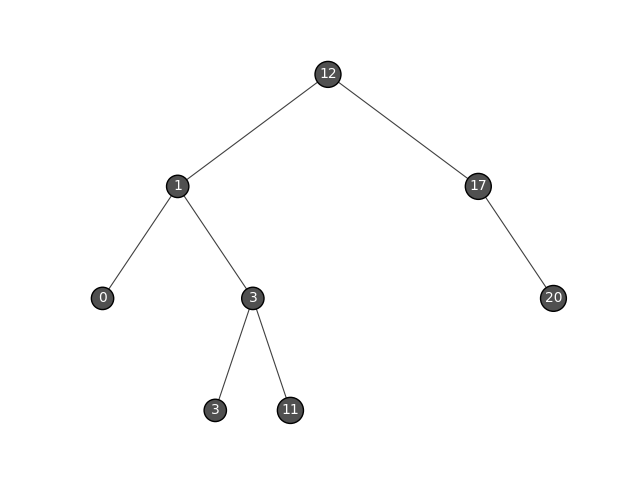
\includegraphics[width=0.7\textwidth]{./images/bst-generic}
  \caption{Esempio di albero binario di ricerca}
  \label{fig:bst-generic}
\end{figure}



\subsection{Cos'è un albero binario di Ricerca?}
Prima di esaminare il problema delle chiavi duplicate cerchiamo di capire cos'è un albero binario di ricerca (abbreviato spesso in B.S.T dall'inglese).
Un BST è un tipo di struttura dati basata su gli alberi, definiti nel libro  \emph{\citefield{cormen2023}{title}} come grafi non orientati, connessi e aciclici. 





\begin{lstlisting}[language=Python, caption={Your Python Code}, label=yourlabel]
# Your Python code here
def hello_world():
    print("Hello, world!")

hello_world()
\end{lstlisting}







\section{Contenuto}
\lipsum[2-3]

\section{Immagini}
\lipsum[4]

\begin{figure}[H]
  \centering
  \includegraphics[width=0.5\textwidth]{example-image-a}
  \caption{Esempio di immagine}
  \label{fig:example}
\end{figure}

\lipsum[5]


\printbibliography


\end{document}
